% ==================================================
\section{Models}
\label{methods:models}
To address the problem of decoding visual stimuli, we implemented several different models. Some were selected as a simple baseline~\ref{methods:models:linear-regression}, and others were based on state-of-the-art CNN networks~\ref{methods:models:CNNv4} for image decoding~\citep{zhang2020reconstruction}. The ones that performed the best are presented in this section. We start this section by properly defining the problem we are solving~\ref{methods:models:problem-definition}.


% **************************************************
\subsection{Problem Definition}
\label{methods:models:problem-definition}
The problem of decoding image stimuli from cortical activity in this thesis is defined as follows. The cortical activity consists of the responses of the neurons in the primary visual cortex to visual stimuli. The goal of the decoding process is to accurately generate a visual stimulus image that is similar to the one presented to the subject based on the recorded cortical activity.

Let us assume that we are provided with a cortical activity encoded as $\#{x} \in \SX$ where $\SX = \mathbb{R}^{n}$ denotes the space of all possible cortical activity encodings using $n$ neurons.
We are trying to predict stimuli $\#{s} \in \SY$, where $\SY = [0;1]^{h \times w}$ denotes space of all possible stimuli images of width $w$ and height $h$. The stimuli images are therefore grayscale and the pixel values are in the range [0;1], where 0 is the darkest and 1 is the lightest value. In our settings, we can assume $w=h$.

The goal is to create a generator $g:\ \SX \rightarrow \SY$ from a space of all such functions $\SG$ which for given cortical activity vector $\#{x} \in \SX$ predicts a decoded stimulus image $\#{s} \in \SY$. Let us first define
\begin{equation}
\label{equation:predictor-loss}
l(\#{s}, g, \#{x}) = \SL(\#{s}, g(\#{x} ; \#\theta))\:,
\end{equation}
% \begin{equation}
% \label{equation:predictor-loss-mean}
% \SL(\#{s}, g(\#{x} ; \#\theta)) = \sum_{i=1, j=1}^{w, h}{\SL_{i,j}(s_{i,j}, g_{i,j}(\#{x} ; \#\theta))} \cdot \frac{1}{w+h}\:,
% \end{equation}
% where $\SL(\#{s}, g(\#{x} ; \#\theta))$ resp. $\SL_{i,j}(s_{i,j})$ is an arbitrary differentiable loss function (image-wise resp. point-wise defined) (find more details about used loss functions in section~\ref{methods:losses}) which given the stimulus $\#{s} \in \SY$ and generated image given by the generator function $g$ returns the loss value. Values $\#\theta$ are the parameters of the generator function. By $f_{i,j}$ we denote pixel value on $i$-th column and $j$-th row of function $f$.

% Due to minimization, we can simplify the formula~\ref{equation:predictor-loss-mean}, we can also omit the parameters of function $g$ for brevity
% \begin{equation}
% \label{equation:simplified-loss}
% \SL(\#{s}, g) = \sum_{i=1, j=1}^{w, h}{\SL_{i,j}(s_{i,j}, g_{i,j})}\:.
% \end{equation}
where $\SL(\#{s}, g(\#{x} ; \#\theta))$ is an arbitrary differentiable loss function (find more details about used loss functions in section~\ref{methods:losses}). Values $\#\theta$ are the parameters of the generator function.


We want such $g \in \SG$, lets denote it $g^* \in \SG$, that minimizes the value $l(\#{s},g,\#{x})$:

\begin{equation}
%\label{equation:predictor}
% l_{min}(\#{x}) = \argmin_{\#{s}\in \SY, g\in \SG}{l(\#{s},g,\#{x})}\:,
\argmin_{\#{s}\in \SY}l(\#{s},g^*,\#{x}) = \argmin_{\#{s}\in \SY, g\in \SG}{l(\#{s},g,\#{x})}\:.
\end{equation}
%  $g^*$ satisfies
% \begin{equation}
% %\label{equation:predictor-loss-mean}
% \argmin_{\#{s}\in \SY}l(\#{s},g^*,\#{x}) = l_{min}(\#{x})\:.
% \end{equation}


We present several CNN models in the following sections to find $g^*$ using only the standard CNN layers -- namely convolutional layers, fully connected layers, convolutional transpose layers, and batch normalization layers. The CNN models use standard ReLU activation function internally and utilize a sigmoid activation function in the final layer, resulting in the output values being constrained within the range of [0, 1], which matches the range of the stimuli images.

We learn the model parameters, and therefore train the model to approximate $g^*$, by minimizing the formula
\begin{equation}
\label{equation:predictor-loss-minimization}
L(\#\theta) = \sum_{j=1}^m{\SL(\#{s}, g(\#{x} ; \#{\theta}))}\:,
\end{equation}
where $\{(\#{x}^j, \#{s}^j) \in (\SX \times \SY) \mid j=1,2,\dots,m\}$ is the training dataset with $m$ training samples.


% **************************************************
\subsection{Linear Regression}
\label{methods:models:linear-regression}
As a simple baseline, linear regression was used based on its deterministic properties to always converge to the same optimum value. The goal of linear regression is to find a linear relationship that best fits the given data.

In simple linear regression, the relationship between the dependent variable Y and the independent variable X is modeled as a straight line. The equation of the line can be written as:

\begin{equation}
Y = \beta_0 + \beta_1 X + \epsilon
\end{equation}

where $\beta_0$ is the intercept, $\beta_1$ is the slope, and $\epsilon$ is the error term which represents the unexplained variability in the data.

The objective of linear regression is to estimate the values of the parameters $\beta_0$ and $\beta_1$ that best fit the data. This is typically done using the method of least squares, which involves minimizing the sum of the squared errors:

\begin{equation}
\sum_{i=1}^{n}(Y_i - \beta_0 - \beta_1 X_i)^2
\end{equation}

where $n$ is the number of observations.

In our case, to be able to use this method, we linearize the stimuli images $\#{s} \in \SY$ from 2D matrices $w \times h$ to vectors of size $w * h$.


% **************************************************
\subsection{CNNv1}
\label{methods:models:CNNv1}
The first neural network presented is a CNN model that generates an image on the latest layer. 

It has a sequential architecture with several transposed convolutional layers with increasing numbers of filters. Each transposed convolutional layer is followed by a batch normalization layer and a ReLU activation function. The final layer is a transposed convolutional layer with a sigmoid activation function that outputs the reconstructed image.

The network has a total of 278,197,825 parameters, all of which are trainable. The architecture is graphically presented on the picture~\ref{img:methods:models:CNNv1}. Since the output is not 110x110px, we use bilinear interpolation to create the proper output size.

\begin{figure}[H]\centering
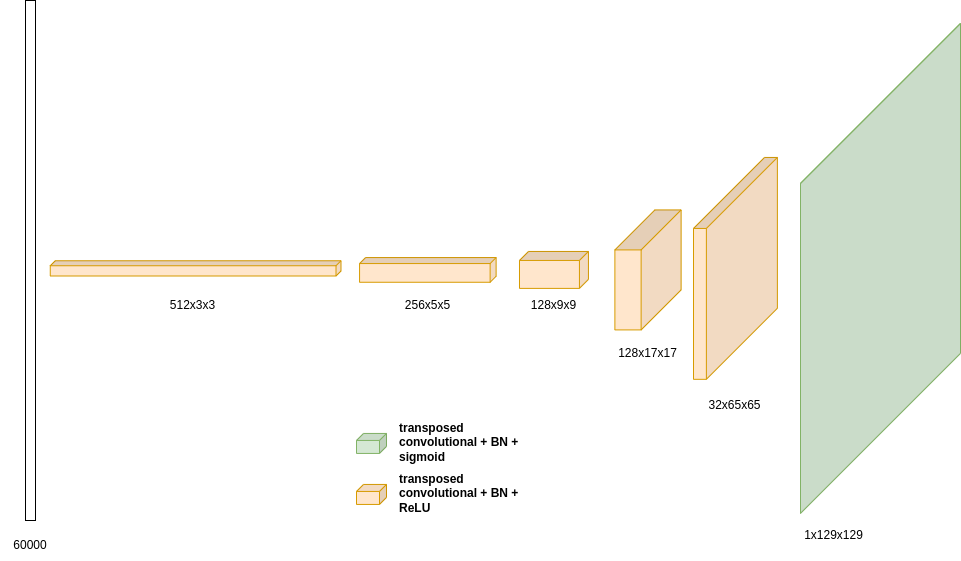
\includegraphics[width=140mm]{img/cnnv1.drawio.png}
\caption{First version of the CNN architecture simply takes the input and uses only transpose convolutional layers without any linear layers to produce the output.}
\label{img:methods:models:CNNv1}
\end{figure}


% **************************************************
\subsection{CNNv2}
\label{methods:models:CNNv2}
The second model is a CNN-based model with a total of 2 sequential parts.

The first part is a fully connected layer consisting of a linear transformation followed by batch normalization, ReLU activation, and dropout. The second part is a sequence of 6 transpose convolutional layers, also known as deconvolutional layers, followed by batch normalization and ReLU activation, and the final layer is a sigmoid activation function. 

The second part of the model takes an input tensor of size [B, 64, 8, 8] and outputs a tensor of size [B, 1, 289, 289], where $B$ is the batch size. The model has a total of 34,695,873 trainable parameters. Since the output is not 110x110px, we again use the same approach by adding bilinear interpolation to create the required output size. The architecture is drawn on picture~\ref{img:methods:models:CNNv2}.

\begin{figure}[H]\centering
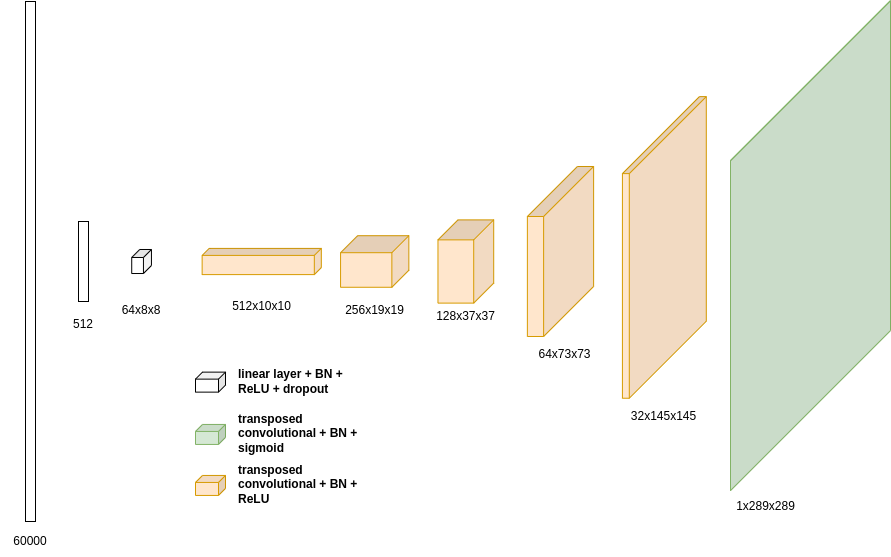
\includegraphics[width=140mm]{img/cnnv2.drawio.png}
\caption{Second version of the CNN architecture. This architecture contains a linear-encoding part and a decoding part producing the final output.}
\label{img:methods:models:CNNv2}
\end{figure}


% **************************************************
\subsection{CNNv3}
\label{methods:models:CNNv3}
The third generative model designed to produce images consists of two main components: a fully connected neural network and a convolutional neural network.

The fully connected network takes a cortical activity vector as input and outputs a 12100-dimensional feature vector. The feature vector is then reshaped into a 110x110px intermediate image tensor and passed through a series of transposed convolutional layers. These layers preserve the spatial dimensions and gradually decrease the channel resolution of the tensor until it has the same dimensions as the desired output image. 

The final layer of the convolutional neural network is a sigmoid activation function that squashes the pixel values of the output image to the range [0, 1]. This property is consistent across all of our models. This model has 38,527,629 trainable parameters and generates images with a size of 110x110 pixels exactly. This architecture is shown in picture~\ref{img:methods:models:CNNv3}.

\begin{figure}[H]\centering
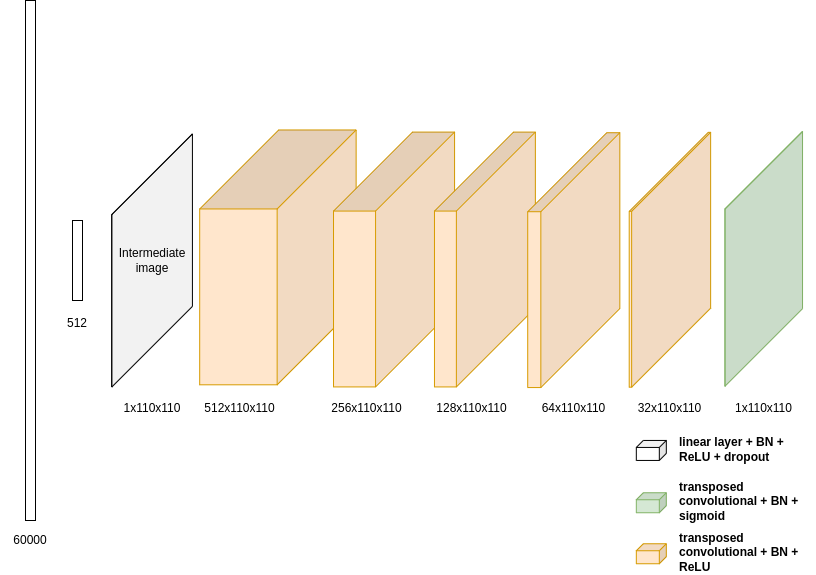
\includegraphics[width=140mm]{img/cnnv3.drawio.png}
\caption{Third version of the CNN architecture. Since the creation of the intermediate image, the dimensions stay the same except for the number of channels.}
\label{img:methods:models:CNNv3}
\end{figure}


% **************************************************
\subsection{CNNv4}
\label{methods:models:CNNv4}
This is a fourth CNN model for image generation, it is an implementation from paper~\citep{zhang2020reconstruction}\footnote{A detailed implementation code in Keras is available at \url{https://github.com/jiankliu/Spike-Image-Decoder/blob/main/SID.py}}. It consists of three sequential blocks. The first block is a fully connected neural network with two linear layers, batch normalization, ReLU activation, and dropout. This produces an intermediate image of size 110x110 pixels with a sigmoid activation function. The second block is a convolutional neural network with four convolutional layers, batch normalization, ReLU activation, and dropout. The third block is an upsampling neural network with four upsampling layers, four convolutional layers, batch normalization, ReLU activation, and dropout.

The input to this model is again a vector of cortical activity, and the output is an image of size 110x110 with each pixel between values 0 and 1. The model is using the sigmoid function as the final activation function to produce the output image. This architecture is drawn on picture~\ref{img:methods:models:CNNv4}.

The model has a total of 37,107,157 parameters out of which 30,720,512 parameters are contained in the first block containing linear layers.

\begin{figure}[H]\centering
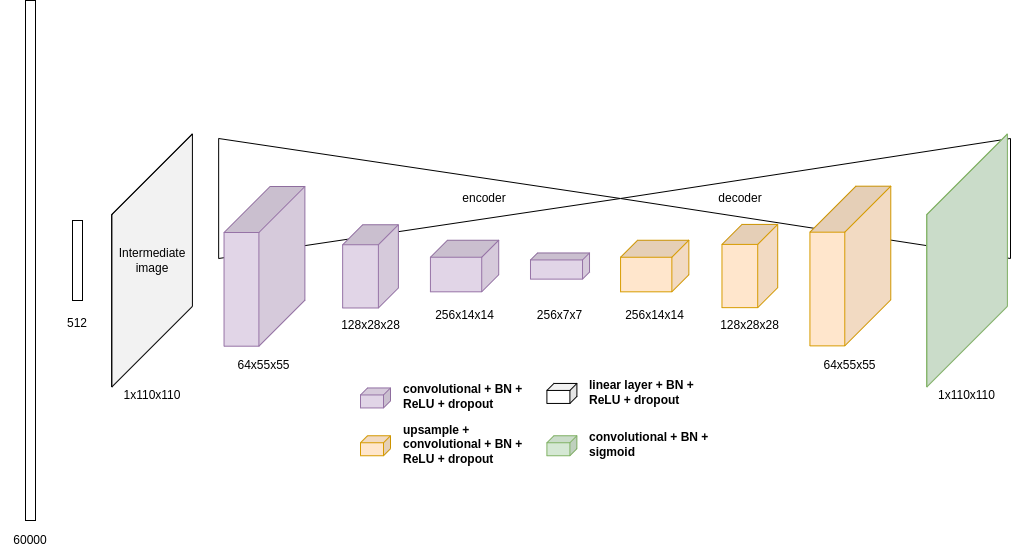
\includegraphics[width=140mm]{img/cnnv4.drawio.png}
\caption{Fourth version of the CNN architecture. The first part producing the intermediate image is here easily distinguishable from the encoder-decoder part of the architecture.}
\label{img:methods:models:CNNv4}
\end{figure}


